\documentclass[UTF8]{EPURapport}
%\usepackage{listings}

%\renewcommand{\lstlistlistingname}{Liste des codes}
%\renewcommand{\lstlistingname}{Code}

%\addextratables{%
%	\lstlistoflistings
%}

%\swapAuthorsAndSupervisors

\thedocument{Cahier d'analyse}{Canne connectée pour aveugles}{}
\grade{Département Informatique\\ 5\ieme{} année\\ 2020-2021}
\authors{%
	\category{Auteurs}{%
		\name{Djawad M'DALLAH MARI} \mail{djawad.mdallah-mari@etu.univ-tours.fr}
	}
	\details{DII5 2020-2021}
}
\supervisors{%
	\category{Encadrants}{%
		\name{Gilles VENTURINI} \mail{gilles.venturini@etu.univ-tours.fr}
	}
	\details{Université François-Rabelais, Tours}
}
\abstracts{Cahier d'analyse canne connecée pour aveugles}
{}
{}
{}

\begin{document}

\chapter{Cahier d'analyse}

\section{Introduction}
Ce cahier d'analyse s'inscrit dans le cadre du projet Canne connectée pour aveugles. Il vise à présenter les analyses faites pour répondre aux besoins exprimés dans le cahier de spécifications. Une lecture au préalable du cahier de spécifications est donc recommandée afin de comprendre le contexte et les enjeux du projet.

Nous verrons donc dans ce document une analyse sur l'application Android à développer. Nous verrons en particulier quelques méthodes de reconnaissances d'objet pour le mobile, la méthode qui sera mise en place pour informer l'utilisateur et également comment garantir à l'utilisateur une interface adaptée à ses contraintes.

\section{Reconnaissance d'objet}
\subsection{Modèles}
L'un des besoins primaire pour la réalisation de ce projet est la reconnaissance d'objet. En effet, toute l’application dépend de la capacité du modèle à détécter et identifier un objet. Afin de répondre à ce besoin, il faudrait faire un inventaire des modèles de reconnaissance d'objet disponible puis faire des comparaisons. Pour mesurer les performances de chaque modèle, des critères doivent être établis ainsi que des conditions de fonctionnement bien défini. Cela permettrait d'avoir un environnement d'exécution commun pour chaque modèle, et donc des mesures cohérentes.

\subsubsection{Modèles disponibles}
Avec la librairie TensorFlow, nous disposons d'un grand panel de modèles pré-entrainés \footnote{\url{https://tfhub.dev}}. Cependant, les modèles adaptés pour TensorFlow Lite restent peu, notamment ceux liés à la reconnaissance d'image et plus particulièrement la reconnaissance d'objets (\textbf{Object Detection}) \footnote{\url{https://tfhub.dev/s?deployment-format=lite&module-type=image-object-detection}}. En effet, il existe que 3 modèles officiels dans cette catégorie : SSD MobileNet, Mobile Object Localizer et East Text Detector. Parmi ces 3, on peut déjà abandonner le East Text Detector puisqu'il s'agit ici de détecter du texte. En revanche, au niveau des modèles de \textbf{Classification}, il existe un peu plus de modèles compatibles TensorFlow Lite \footnote{\url{https://tfhub.dev/s?deployment-format=lite&module-type=image-classification}}.

\newpage

\subsubsection{Object Detection vs Classification}
Les modèles de reconnaissances d'objet (Objet Detection) sont capables de localiser et identifier plusieurs objets sur une même image.

\begin{figure}[h!]
\centering
  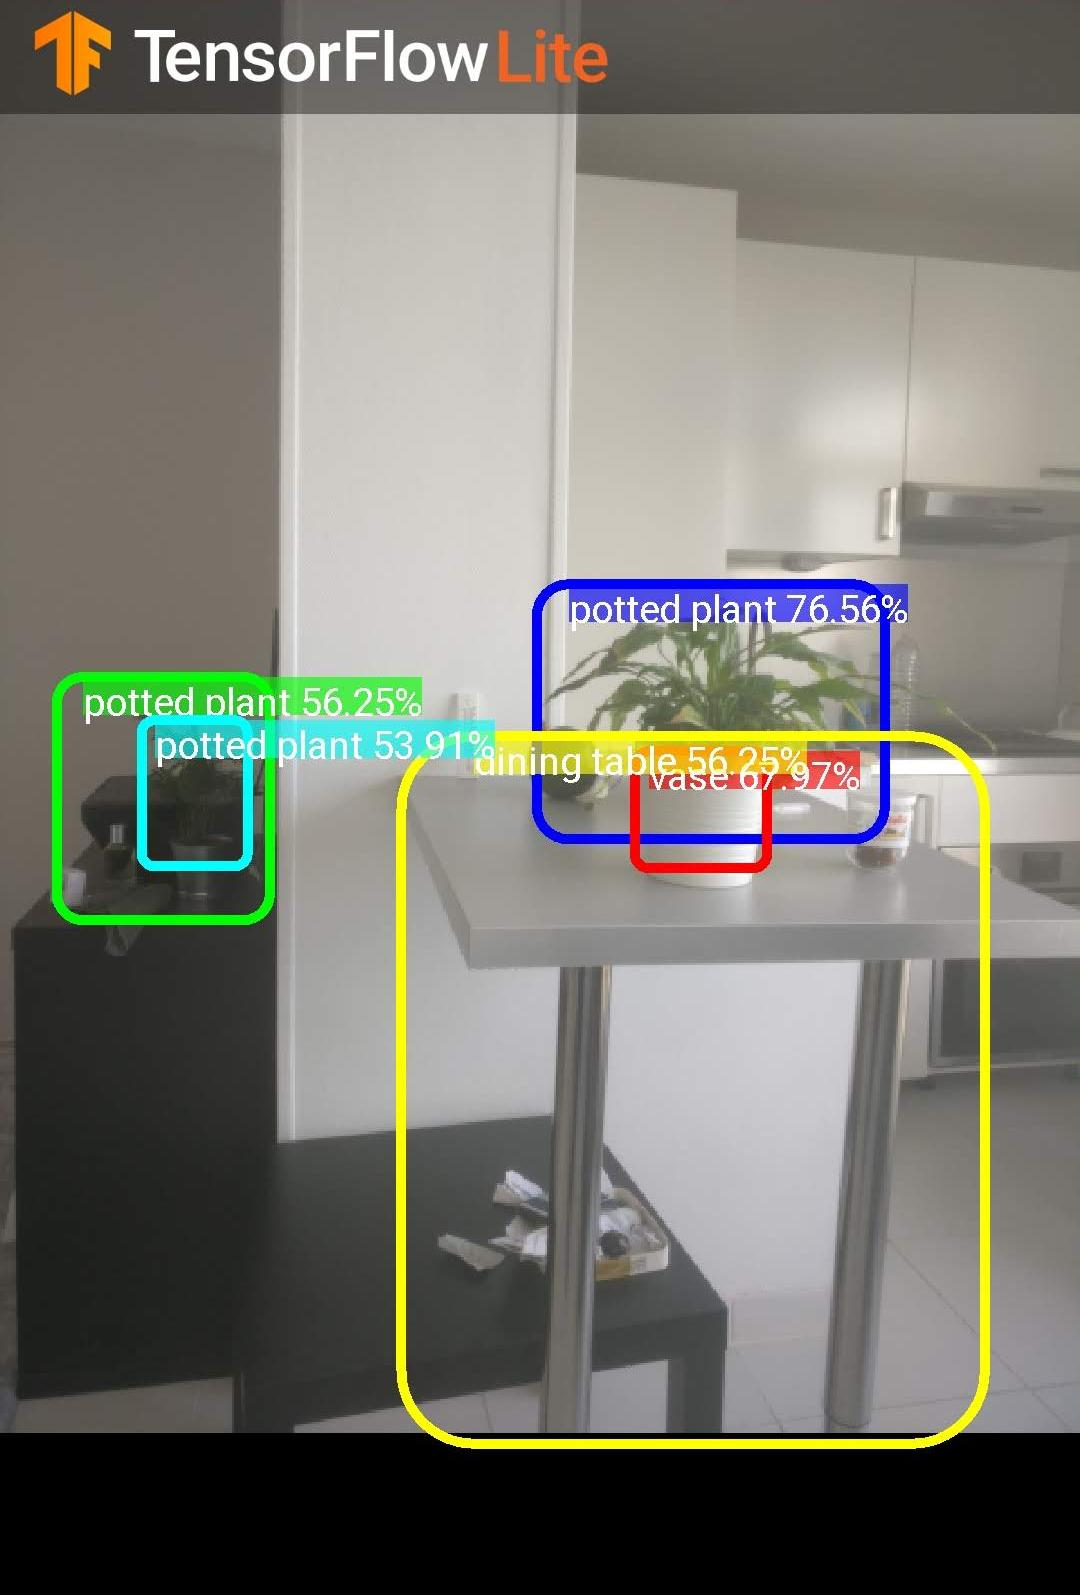
\includegraphics[width=0.5\textwidth]{images/object_detection.jpg}
  \caption{Exemple de reconnaissance d'objet}
  \label{fig:objectdetection}
\end{figure}

 Ce type de modèle est entraîné avec des objets de différents classes (vêtements, fruits, etc.). Avec TensorFlow lorsqu'on met à l'éntrée de ce type de modèle une image, on obtient en sortie une liste d'objets avec chacun sa localisation, sa classe et un degré de confidence (qui correspond à la fiabilité de l'objet identifié).

\begin{figure}[h!]
\centering
  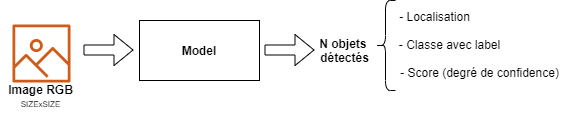
\includegraphics[width=0.6\textwidth]{images/schema_objectDetection.png}
  \caption{Schema principe de fonctionnement d'un modèle}
  \label{fig:schema_objectdetection}
\end{figure}

En revanche, les modèles de classification avec TensorFlow ne détecte qu'un seul élément sur une image. Ces modèles sont entrainés sur une seule classe générique (exemple : vêtements, aliments, plantes, etc) qui va ensuite être capable d'identifier l'élément de manière plus précise. Exemple : \\

\begin{itemize}
  \item Classe vêtements : T-shirt, jean, ...
  \item Classe aliments : salade, pâtes, ...
  \item Classe fruits : pomme, banane, ...  
  \item Classe insectes : sauterelle, abeille, papillon, ...
  \item  ...
\end{itemize}

\begin{figure}[h!]
\centering
  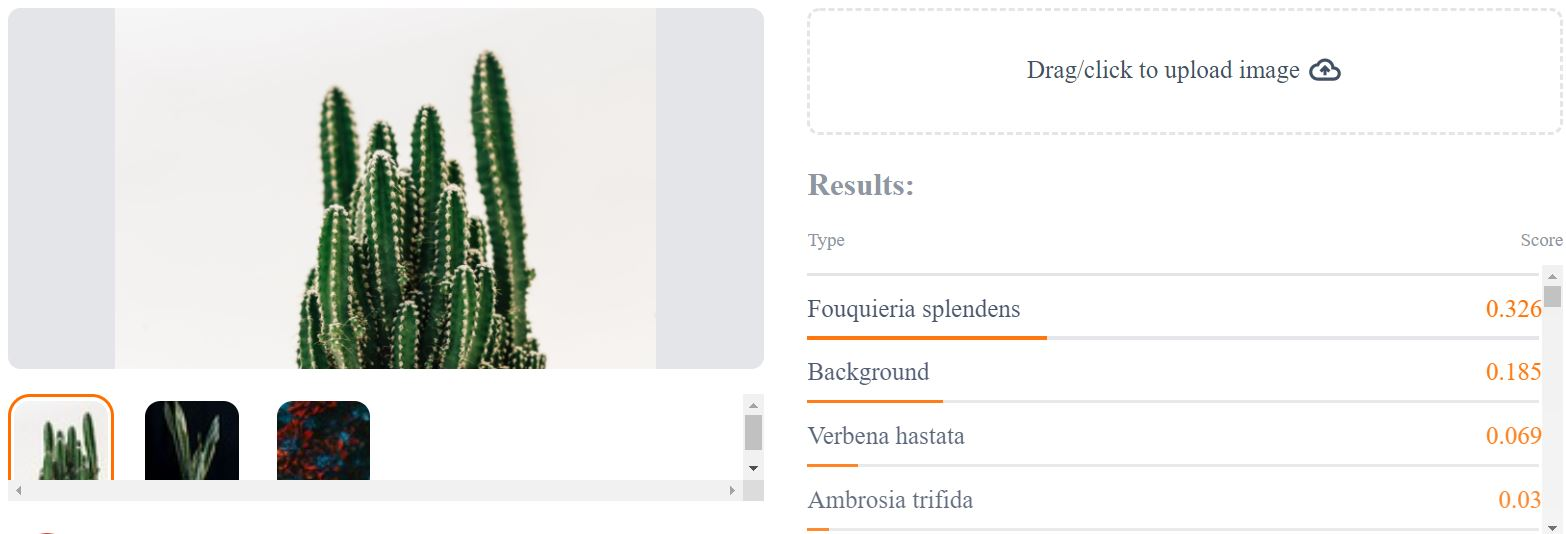
\includegraphics[width=\textwidth]{images/plants_classification.jpg}
  \caption{Exemple de classification de plantes}
  \label{fig:plantsclassification}
\end{figure}

\subsubsection{Choix du modèle}

classification
banque d'image
Dans notre cas 
benchmark..
id 1 objet à la X(objet id)
\subsection{Intégration dans une application Android}
les méthodes d'integration
fonctionnement
entrée sortie

\section{Informer l'utilisateur}
\subsection{Synthèse vocale}
fonctionnement
parametrage
rendre le message compréhensible: viseur,
vibreur
encodage-trame (1mots,phrase,1vib,2vib,vib long..?)
diag de classe

\subsection{Vibration}

\section{Navigation}
\subsection{Guide d'utilisation}
\subsection{Accès aux réglages}

\annexes

\end{document}